\section{Chain D -- ZBEE\_ZCL Handler (output 1 of router)}

Builds the prescribed publish payload, rate-limits it to 10\,msg/min
and publishes it to a topic named after the ZigBee source device. The
same message is parsed for RMS Current / RMS Voltage / Active Power
attributes and forwarded to \texttt{filtered\_elems.csv} and to two
dashboard charts.

\begin{figure}[h]
    \centering
    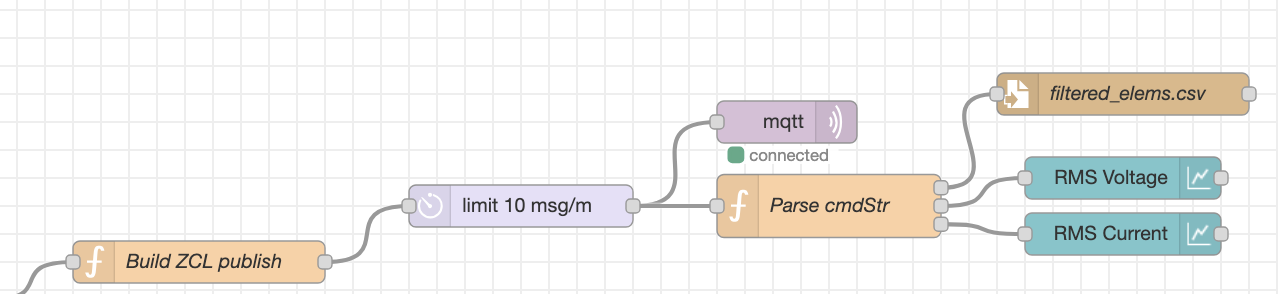
\includegraphics[width=\linewidth]{images/flow_chain_d.png}
    \caption{Chain D -- ZCL publish, filtering and charts.}
\end{figure}

\begin{description}
    \item[Function \emph{Build ZCL publish}] reads the cached row,
        assembles the JSON payload mandated by the specification and
        stores the dynamic topic name (\texttt{Device Name ZigBee
        Source}) in \verb|msg.topic|. The character \texttt{+} is
        stripped from the topic because it is reserved by the MQTT
        protocol as a single-level wildcard and would otherwise be
        rejected by the broker (e.g.\ \texttt{Ledvance Smart+ Plug}).
        \begin{lstlisting}[]
        const lookup = msg.lookup;
        const row = lookup.row;
        const subId = lookup.subId;
        
        const srcAddr     = row["Source Address"];
        const dstAddr     = row["Destination Address"];
        const zbSrcAddr   = row["Source Address ZigBee"];
        const zbDstAddr   = row["Destination Address ZigBee"];
        const zbSrcNameRaw = row["Device Name ZigBee Source"] || "";
        const zbSrcName    = zbSrcNameRaw.replace(/\+/g, "");
        const cmdStr      = row["Command String"] || "";
        
        const payload = {
            timestamp: Math.floor(Date.now() / 1000),
            id: subId,
            "wpan.src": srcAddr,
            "wpan.dst": dstAddr,
            "zbee.src": zbSrcAddr,
            "zbee.dst": zbDstAddr,
            topic: "ZigBee/" + zbSrcName,
            payload: cmdStr
        };
        
        msg.payload = payload;
        msg.topic = zbSrcName;
        return msg;
        \end{lstlisting}
    \item[Delay (\emph{rate limit, 10/min})] queues messages and
        releases at most ten per minute, with no intermediate drops.
    \item[MQTT out (dynamic topic)] empty \emph{Topic} field, so the
        broker uses \verb|msg.topic| at runtime.
    \newpage
    \item[Function \emph{Parse cmdStr}] converts the
        Python-dictionary-style Command String into a JSON object by
        replacing single quotes with double quotes, walks the parallel
        arrays \texttt{Attribute}/\texttt{Status}/\texttt{Data Type} and
        consumes one value at a time from the corresponding typed list
        (\texttt{Int16}, \texttt{Uint16}, \dots) using a per-type
        cursor. Only entries whose attribute is one of the three
        targets \emph{and} for which all of \texttt{Status},
        \texttt{Data Type} and value are populated are retained;
        everything else is discarded, which in practice removes
        \texttt{Read Attributes} \emph{request} packets (no value) and
        spontaneous reports lacking a status. The node has three
        outputs: the CSV chunk, the RMS Voltage chart messages and the
        RMS Current chart messages.
        \begin{lstlisting}[]
        const cmdStr = msg.lookup.cmdStr;

        // Quick reject
        if (!cmdStr.includes("RMS Current") &&
            !cmdStr.includes("RMS Voltage") &&
            !cmdStr.includes("Active Power")) {
            return null;
        }
        
        // Python-dict to JSON
        let obj;
        try {
            obj = JSON.parse(cmdStr.replace(/'/g, '"'));
        } catch (e) {
            node.warn("Parse failed: " + e.message);
            return null;
        }
        // normalize a value to an array
        const arr   = (v) => v === undefined ? [] : Array.isArray(v) ? v : [v];
        // an input like "RMS Voltage (0x0505)" becomes "RMS Voltage"
        const clean = (s) => String(s).replace(/\s*\(0x[0-9a-fA-F]+\)\s*$/, "").trim();
        // extract the leading integer "230 V" becomes "230"
        const num   = (s) => { const m = /^(-?\d+)/.exec(String(s)); return m ? m[1] : String(s); };
        
        const typeMap = {
            "16-Bit Signed Integer":   "Int16",
            "16-Bit Unsigned Integer": "Uint16",
            "8-Bit Signed Integer":    "Int8",
            "8-Bit Unsigned Integer":  "Uint8",
            "32-Bit Signed Integer":   "Int32",
            "32-Bit Unsigned Integer": "Uint32",
        };
        
        const attributes = arr(obj.Attribute);
        const statuses   = arr(obj.Status);
        const dataTypes  = arr(obj["Data Type"]);
        const cursor     = {};
        
        const ts     = msg.payload.timestamp;
        const seqNum = obj["Sequence Number"] || "";
        
        const csvLines = [];
        const voltMsgs = [];
        const currMsgs = [];
        let rowNum = flow.get('filteredRowNum') || 0;
        
        // Walk through every attribute. The values aren't stored
        // alongside their attribute names — they're grouped by data type into
        // separate arrays (Int16, Uint16, etc.). The `cursor` object tracks how
        // many values of each type are already consumed, so on each iteration
        // we pull the *next* value of the matching type.
        for (let i = 0; i < attributes.length; i++) {
            const attrName      = clean(attributes[i]);
            const dataTypeLabel = clean(dataTypes[i] || "");
            const tf            = typeMap[dataTypeLabel];
        
            let value = "";
            if (tf) {
                const list = arr(obj[tf]).map(num);
                const idx  = cursor[tf] || 0;
                value      = list[idx] !== undefined ? list[idx] : "";
                cursor[tf] = idx + 1;
            }
        
            if (attrName !== "Active Power" &&
            attrName !== "RMS Current" &&
            attrName !== "RMS Voltage") continue;
        
            const status   = statuses[i] ? clean(statuses[i]) : "";
            const dtLabel  = clean(dataTypes[i] || "");
        
            if (value === "" || !status || !dtLabel) continue;
        
            rowNum++;
            if (rowNum === 1) {
                csvLines.push("No.,Timestamp,Sequence Number,Attribute,Status,Data Type,Data Value");
            }
            csvLines.push(`${rowNum},${ts},${seqNum},${attrName},${status},${dataTypeLabel},${value}`);
        
            if      (attrName === "RMS Current") currMsgs.push({ payload: Number(value), topic: "RMS Current" });
            else if (attrName === "RMS Voltage") voltMsgs.push({ payload: Number(value), topic: "RMS Voltage" });
        }
        
        flow.set('filteredRowNum', rowNum);
        
        if (csvLines.length === 0) return null;
        
        return [
            { payload: csvLines.join("\n") + "\n" },
            voltMsgs.length ? voltMsgs : null,
            currMsgs.length ? currMsgs : null
        ];
        \end{lstlisting}
    \item[File (append)] writes the CSV chunk to
        \texttt{filtered\_elems.csv}.
    \item[Chart \emph{RMS Voltage} / \emph{RMS Current}] two
        node-red-dashboard line charts on the same UI group.
\end{description}

\begin{figure}[h]
    \centering
    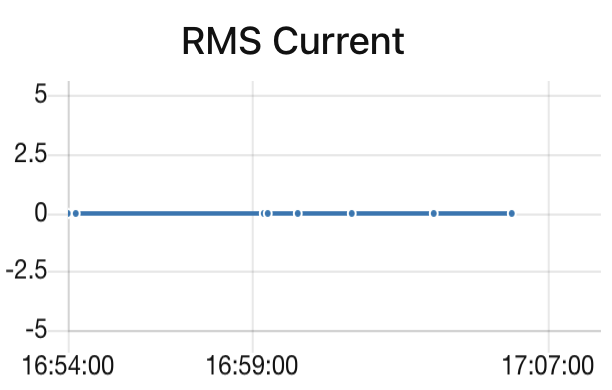
\includegraphics[width=0.45\linewidth]{images/chart_rms_current.png}
    \hfill
    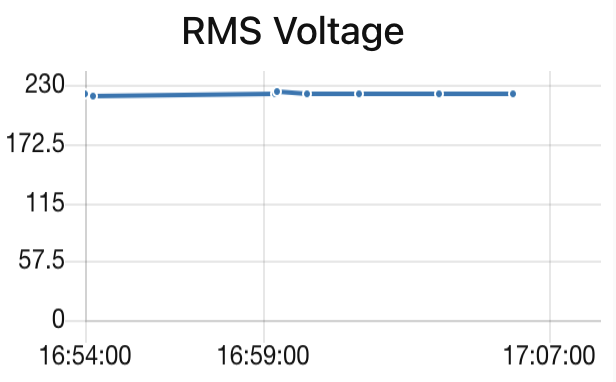
\includegraphics[width=0.45\linewidth]{images/chart_rms_voltage.png}
    \caption{Live charts of RMS Current and RMS Voltage.}
\end{figure}